\chapter*{Introduzione}
Una \textbf{moneta virtuale} è, fondamentalmente, uno strumento utilizzato per effettuare transazioni all'interno di un ecosistema digitale. Per comprenderne a pieno la natura e le sfide tecnologiche, è essenziale confrontarla prima con la moneta tradizionale (reale).

Le monete reali possiedono un valore che deriva storicamente da due paradigmi principali:
\begin{itemize}
    \item \textbf{Valore Intrinseco:} Basato sulla scarsità e sulle proprietà del materiale stesso (come nel caso dell'oro). Generare una copia di un bene con valore intrinseco ha un costo equivalente al valore del bene stesso.
    \item \textbf{Valore Stabilito:} Il valore della banconota è imposto e garantito da un'autorità centrale, come una Banca Centrale. In questo caso, per mantenere il valore della valuta, la sua riproduzione \textbf{falsificazione} deve essere resa artificialmente complessa, affinché il costo, la difficoltà o il rischio di creare una copia eguagli o superi il valore nominale della moneta stessa.
\end{itemize}

Passando al mondo informatico, il paradigma cambia radicalmente: fare copie di un dato digitale è un'operazione estremamente semplice e a costo quasi zero. Di conseguenza, impedire la riproduzione non autorizzata e la spesa multipla della stessa moneta virtuale rappresenta una sfida tecnologica notevole, nota in informatica come il problema del \textit{double-spending} (o doppia spesa).

Nei sistemi di pagamento digitale tradizionali, come le carte di credito o i bonifici online, la soluzione a questo problema non risiede nella natura del dato digitale in sé. Piuttosto, il sistema si affida a \textbf{TTP (Trusted Third Parties - Enti Terzi Fiduciari)}, ovvero banche, istituti finanziari o circuiti di pagamento. Questi enti centralizzati non si limitano semplicemente a "inviare dati digitali", ma fungono da garanti assoluti: gestiscono i registri contabili, verificano le disponibilità e si occupano di tutta l'infrastruttura amministrativa e burocratica (le classiche "scartoffie") che lega e converte il dato virtuale alla valuta reale corrispondente.

È in questo contesto che si inserisce la rivoluzione del \textbf{Bitcoin}. Ideato nel 2008 sotto lo pseudonimo di \textbf{Satoshi Nakamoto}, Bitcoin nasce con il preciso obiettivo di superare i limiti strutturali legati alla necessità di fiducia e alla centralizzazione dei sistemi tradizionali. 

Le sue caratteristiche fondanti, che lo distinguono dalle precedenti monete virtuali, sono:
\begin{itemize}
    \item \textbf{Assenza di TTP:} Non esiste un'autorità centrale, un server principale o un ente terzo fiduciario incaricato di validare le transazioni o emettere nuova moneta.
    \item \textbf{Sistema Distribuito:} La validazione delle transazioni e la tenuta dei registri avvengono in modo decentralizzato tramite un network \textit{peer-to-peer}, supportato da una struttura dati pubblica chiamata Blockchain.
    \item \textbf{Pseudo-anonimato:} Gli utenti operano e scambiano valore tramite indirizzi crittografici, senza la stretta necessità di associare un'identità anagrafica diretta per poter partecipare al network.
    \item \textbf{Accessibilità ed Efficienza:} Fin dalla sua concezione, e in particolare nelle sue prime fasi storiche, il protocollo ha dimostrato la possibilità di effettuare transazioni globali, incensurabili e a costi estremamente ridotti rispetto ai circuiti interbancari internazionali.
\end{itemize}

\chapter{Funzioni Hash}
Una funzione Hash è una funzione che prende in input una stringa di lunghezza arbitraria e ritorna in un output una stringa di lunghezza fissata che, nel nostro caso, sarà una stringa di 256 bit. Questa funzione gode di tre proprietà fondamentali:
\begin{itemize}
    \item \textbf{Collision-Resistant:} Ossia non è possibile per avversari computazionalmente limitati trovare due input $x$ e $y$ tali che il $H(x) = H(y)$.
    \item \textbf{Hiding:} Diciamo che la funzione Hash gode della proprietà di Hiding poiché è computazionalmente intrattabile trovare a partire da $H(x)$ il valore x. Inoltre, è anche impossibile a partire da $H(x|r)$ cosa non è $x$, evitando quindi attacchi di brute force. 
    \item \textbf{Puzzle-Friendly:} Questa proprietà delle funzioni hash fa' sì che noi possiamo trasformarle in una sorta di puzzle o sfida. In pratica, quello che faremo sarà fissare dei dati k e aggiungeremo una randomness $x$ tale che $H(k|x) = y$ con y che una certo pattern. Questo pattern è, in genere, un certo numero di zeri all'inizio alla fine dell'hash e, maggiori sono gli zeri che vogliamo, maggiore sarà la difficoltà. Esattamente come un puzzle, sarà "difficile" da risolvere ma facile da verificare.
\end{itemize}
Queste proprietà sono fondamentali per implementare uno schema di \textbf{Commitment}. Possiamo immaginare il commitment come l'equivalente digitale del mettere un messaggio in una busta sigillata e lasciarla in bella vista sul tavolo: tutti possono vedere la busta (il valore è "pubblicato" e quindi non può più essere modificato), ma nessuno può verificarne il contenuto finché non decidiamo di aprirla. Formalmente, questo meccanismo si articola in due fasi, gestite da altrettanti algoritmi:
\begin{itemize}
    \item \textbf{Fase di Commit:} L'algoritmo prende in input il messaggio $m$ che vogliamo vincolare e un valore casuale $r$ (necessario per garantire la proprietà di \textit{hiding}). Restituisce in output il commitment $com$, ovvero la nostra "busta chiusa". Da questa stringa $com$ è computazionalmente impossibile risalire alla coppia $(m, r)$.
    \item \textbf{Fase di Reveal e Verifica:} Quando si decide di svelare l'informazione, vengono resi pubblici $m$ e $r$. A questo punto interviene l'algoritmo di $Verify$, che riceve in input i valori $com$, $m$ e $r$. Esso calcola internamente $Commit(m, r)$ e restituisce $1$ (Vero) se il risultato corrisponde esattamente al $com$ pubblicato in precedenza, oppure $0$ (Falso) altrimenti. Questo garantisce la certezza matematica che il messaggio non sia stato alterato dopo la sua pubblicazione.
\end{itemize}

\section{Hash Pointers e Struttura della Blockchain}

Da un punto di vista strutturale, una Blockchain può essere concettualmente assimilata a una \textit{linked list} (lista concatenata). A differenza delle liste tradizionali, però, essa utilizza dei \textbf{Hash Pointers} (puntatori hash). Un hash pointer non si limita a indicare dove recuperare l'elemento precedente, ma contiene anche l'hash crittografico dei dati di quel blocco.\footnote{È importante notare che l'hash crittografico di per sé non è un indirizzo di memoria fisico o di rete; nei sistemi reali (come nei nodi Bitcoin), il client utilizza l'hash come chiave per cercare e recuperare il blocco corretto all'interno del proprio database locale.}

In una blockchain, ogni blocco contiene l'hash pointer al blocco \textbf{precedente}. Grazie a questo meccanismo, la catena diventa un registro a prova di manomissione \textit{tamper-evident}: ogni blocco si fa garante dell'integrità di tutta la cronologia passata. Modificare anche un solo bit all'interno di un blocco altererebbe inevitabilmente il suo hash, rompendo la validità del puntatore nel blocco successivo e generando un effetto a cascata che invaliderebbe l'intera catena da quel punto in poi. L'unico modo per mascherare un attacco del genere sarebbe trovare una collisione nella funzione hash ma, come già discusso, per funzioni sicure ciò è computazionalmente intrattabile.

\begin{figure}[H]
    \centering
    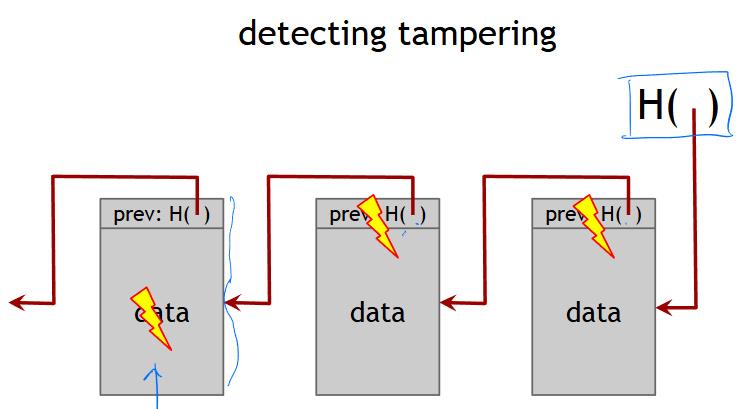
\includegraphics[width=0.5\linewidth]{Images/capitolo_1/tampering_block.png}
\end{figure}

\subsection{Il Merkle Tree}
All'interno di ogni singolo blocco, le transazioni (i dati) non sono semplicemente elencate, ma sono organizzate utilizzando un'altra struttura basata sugli hash pointers: il \textbf{Merkle Tree} (Albero di Merkle). 

Si tratta di un albero binario costruito con un approccio \textbf{bottom-up}:
\begin{itemize}
    \item Le \textbf{foglie} dell'albero contengono gli hash delle singole transazioni.
    \item Ogni \textbf{nodo padre} viene generato concatenando gli hash dei suoi due figli e calcolandone a sua volta l'hash (es. $H(H(A) \parallel H(B))$).
\end{itemize}
Questo processo si ripete e si restringe fino a ottenere un unico hash radice, chiamato \textbf{Merkle Root}, che rappresenta crittograficamente tutte le transazioni e viene inserito nell'intestazione (header) del blocco. 

Essendo costruito dal basso verso l'alto, l'albero risulta bilanciato. Questa struttura è estremamente efficiente poiché permette di verificare se una specifica transazione è inclusa in un blocco richiedendo solo il percorso dalla foglia alla radice (la cosiddetta \textit{Merkle Proof}). Questo approccio abbatte i costi computazionali e di memoria, consentendo verifiche con una complessità logaritmica ($O(\log n)$).

\begin{figure}[H]
    \centering
    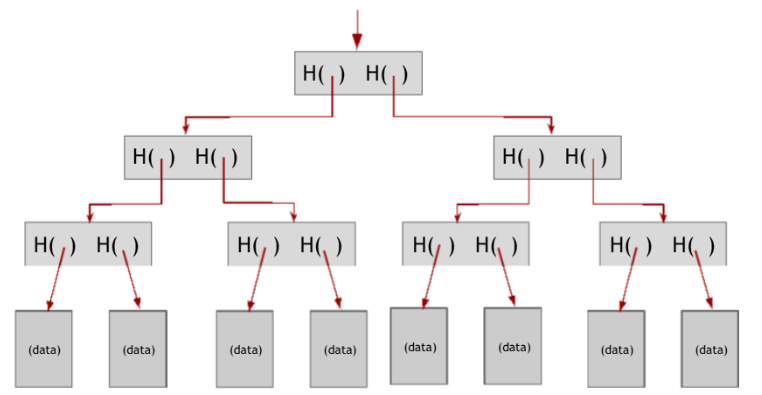
\includegraphics[width=0.5\linewidth]{Images/capitolo_1/Merkle_tree.png}
\end{figure}

\subsubsection*{Verifica di inclusione: La Merkle Proof}
Una delle caratteristiche più potenti del Merkle Tree è la possibilità di verificare se una specifica transazione è inclusa in un blocco senza dover scaricare o scorrere l'intero albero. Questo meccanismo, noto come \textbf{Merkle Proof}, è alla base del funzionamento dei nodi leggeri (SPV - \textit{Simplified Payment Verification}).

Per effettuare questa verifica, a un client sono necessari solo tre elementi:
\begin{enumerate}
    \item L'\textbf{hash della transazione} che si vuole verificare (la foglia di partenza).
    \item La \textbf{Merkle Root}, che è pubblicamente disponibile nell'header del blocco.
    \item Il \textbf{Merkle Path} (o percorso di prova), ovvero la lista degli hash dei nodi "fratelli" necessari per risalire l'albero fino alla radice.
\end{enumerate}

\textbf{Il processo di verifica:}
Il client calcola l'hash della propria transazione e lo concatena con il primo hash fornito nel Merkle Path (il nodo fratello), calcolando il nuovo hash padre. Questo procedimento viene ripetuto iterativamente, salendo di livello in livello, fino a ottenere un singolo hash finale. 
Se l'hash calcolato dal client \textbf{coincide esattamente} con la Merkle Root del blocco, si ha la certezza crittografica che la transazione è valida e regolarmente inserita nel blocco. Poiché l'albero è binario, la quantità di hash fratelli da richiedere (il Merkle Path) cresce in modo logaritmico rispetto al numero totale di transazioni ($O(\log n)$), garantendo un'enorme efficienza in termini di banda e computazione.

\section{Firma digitale}
Una firma digitale è l’equivalente informatico di una tipica firma convenzionale. La struttura è molto simile a quella del Message Authentication, tuttavia qui abbiamo
una struttura simmetrica in cui abbiamo una \textbf{chiave segreta che serve a firmare} e una \textbf{chiave pubblica che serve per verificare}.
Uno schema di firma digitale è composto da tre algoritmi
\begin{enumerate}
    \item \textbf{generateKeys:} algoritmo che genera la chiave di verifica che sarà pubblica e la chiave di firma che sarà privata. È importante notare che Bitcoin garantisce "pseudoanonimato" poiché anziché usare la propria identità, le transazioni avvengono tramite la chiave di verifica. Dunque, non abbiamo un riferimento diretto all'identità e, inoltre, a ogni persona potrebbero corrispondere infinite coppie di chiavi.
    \item \textbf{sign:} è l'algoritmo che ci permetter di firmare le transazioni.
    \item \textbf{verify:} algoritmo che controlla che una certa firma sia valida
\end{enumerate}

In particolare, lo schema di firma adottato da Bitcoin è \textbf{ECDSA} uno schema di firma particolarmente efficace che sfrutta punti di curve ellittiche per permettere una cifratura sicura con chiavi crittografiche a soli 256 bit. Per semplicità, spiegheremo lo schema DSA che è praticamente lo stesso di ECSDA ma usa spazi $Z_N^*$ anziché curve ellittiche. Questo schema di firma si basa sul problema del \textbf{logaritmo discreto} che consiste nel problema del non riuscire a ricavare in tempo efficiente quel valore $x:g^x = X$ dati solo $X$ e $g$. Gli algoritmi di firma e verifica sono dunque:
\begin{figure}[H]
    \centering
    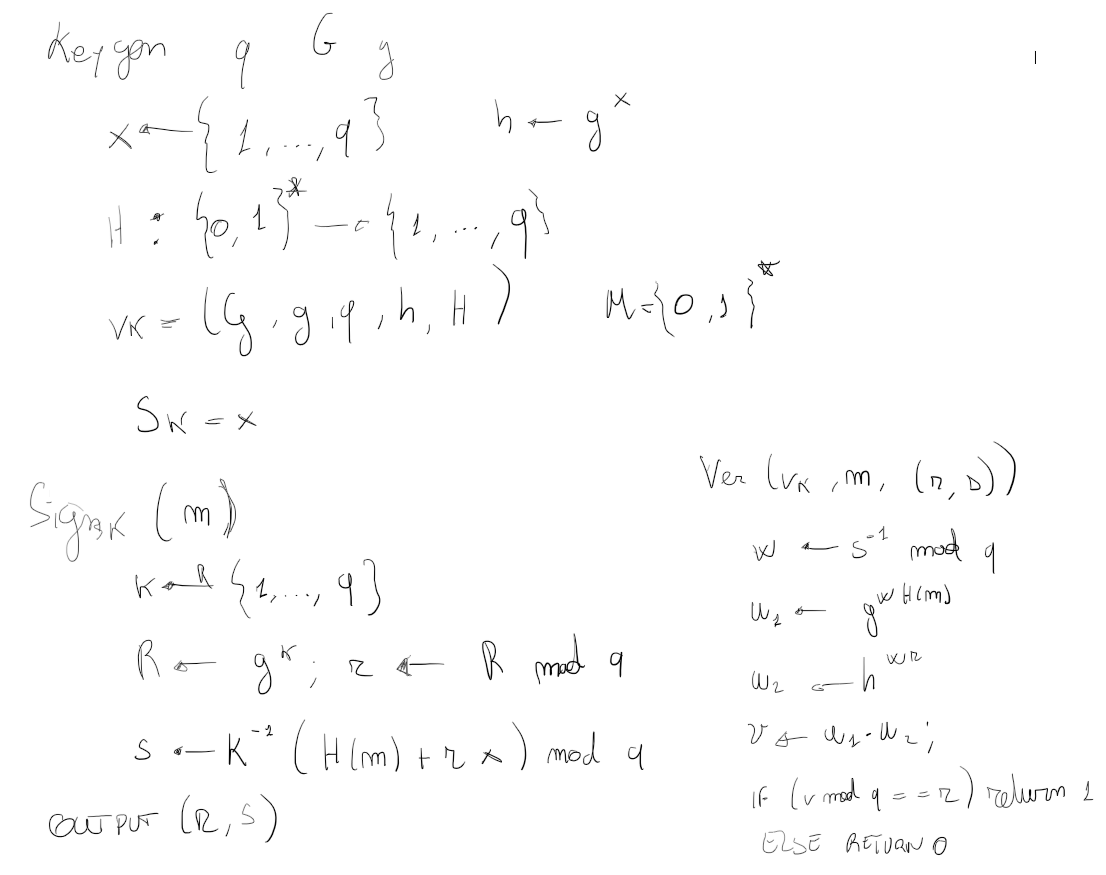
\includegraphics[width=0.7\linewidth]{Images/capitolo_1/ecdsa.png}
\end{figure}
Come già detto tutto fa riferimento alle chiavi pubbliche che saranno le identità chiamate \textbf{indirizzi} in Bitcoin.

\section{Basic Cryptocurrencies}
Vediamo adesso una carrellata di Cryptocurrencies basilari utili a mostrare tutte le problematiche di implementare delle monete digitali.

\subsection{GoofyCoin}
Immaginiamo questa moneta che possiede le seguenti operazioni o \textbf{transazioni}:
\begin{itemize}
    \item \textbf{CreateCoin(uniqueCoinID):} Questa operazione permette di creare una nuova moneta e, banalmente, colui che effettua questa transazione la firma con la sua chiave privata. Così facendo, tutti possono verificare che quella moneta gli appartiene.
    \item \textbf{PayTo(indirizzo):} Questa operazione permette a qualcuno di pagare una moneta (in questo momento unitaria) a un altro indirizzo. Per farlo, oltre a fornire l'indirizzo a cui inviare la moneta, è necessario fornire l'hash pointer del blocco contente la transazione di creazione o dell'avvenuto ricevimento della moneta.
\end{itemize}
Questo schema, seppur basilare, ci è utile a mostrare il problema del \textbf{double spending}, infatti, poiché l'unica cosa necessaria da fornire per un pagamento è un'hash pointer che provi che ci appartiene quella specifica moneta, ci basta fare tutti i pagamenti con lo stesso punto di partenza. Così facendo, riusciremo a spendere infinite volte la stessa moneta.
\begin{figure}[H]
    \centering
    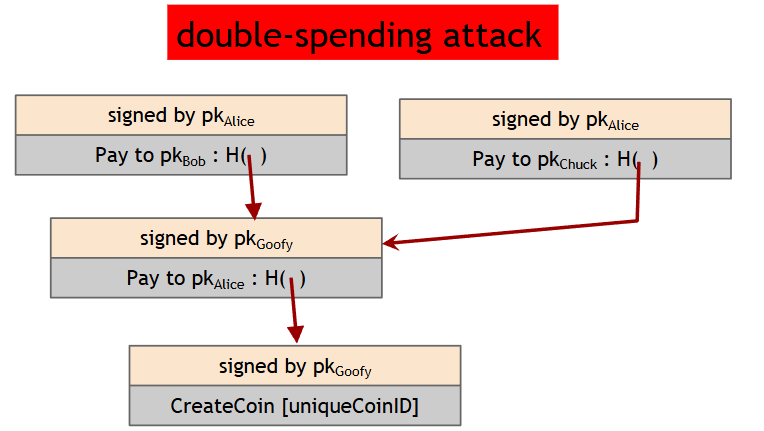
\includegraphics[width=0.7\linewidth]{Images/capitolo_1/double_spending.png}
\end{figure}

Inoltre, un altro problema è che allo stato attuale, \textbf{ognuno può creare la sua moneta gratis} e che, all'aumentare di scambi della moneta, si vanno a creare delle \textbf{catene di verifica sempre più grandi}.

Tutti questi problemi nascono dal fatto che abbiamo un sistema del tutto \textbf{decentralizzato}. Passiamo dunque alla prossima tipologia di moneta.

\subsection{ScroogeCoin}
A differenza della moneta precedente, immaginiamo di voler creare un sistema completamente centralizzato. Poiché centralizzato, questo sistema sarà \textbf{controllato da un'unica entità} che, in questo caso, sarà "Zio Paperone". Questa entità sarà l'unica a poter creare nuova moneta e a gestire il registro (cioè la Blockchain) e, quindi, decidere quali operazioni inserire e quali no.
\begin{figure}[H]
    \centering
    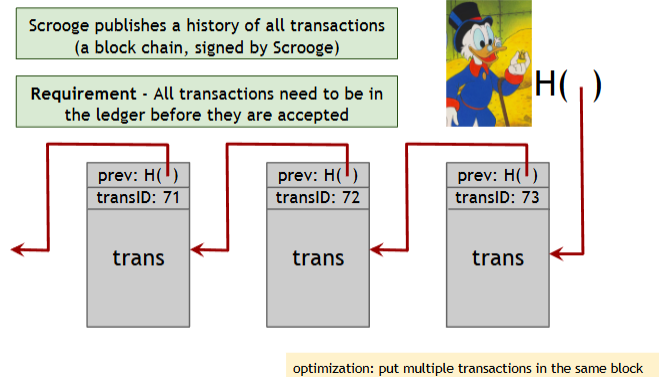
\includegraphics[width=0.7\linewidth]{Images/capitolo_1/scrooge_coin.png}
\end{figure}
Inoltre, anziché fare pagamenti unitari, possiamo spezzettare i pagamenti facendo sì che, ad esempio, se l’unità è 100 euro, per pagare un caffè pago 1 euro al commerciante e 99 euro a me stesso. Naturalmente ciò complica le cose perché si devono fare tante verifiche, tuttavia è fattibile. 

Eliminiamo anche il problema del double spendig poiché, essendo l'entità a decidere quali operazioni accettare e quali no sul registro e, dunque, non permetterebbe mai una cosa del genere\dots

Tutto ciò accade se e solo se l'entità non è malevola, in caso contrario, nessun potrebbe contrastarla, rendendo inutilizzabile la moneta.

